\documentclass{ximera}

\title{Practice}

\begin{document}
\begin{abstract}
  Try these problems.
\end{abstract}
\maketitle




\begin{exercise}

%%{Calculate limits from a graph (or state that the limit does not exist).}
%%{Explain the relationship between one-sided and two-sided limits.}
%%{Distinguish between limit values and function values.}
%%{Identify when a limit does not exist.}



%%{limit} 


Let $f$ be defined on the interval $\left[0,2\right]$, and no where else, whose graph is:
\begin{image}
 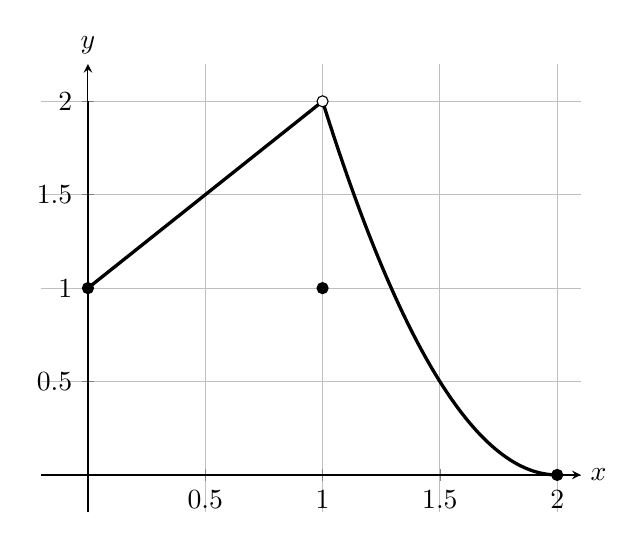
\begin{tikzpicture}
	\begin{axis}
	[ymin=-0.2,ymax=2.2, axis lines=center,xlabel=$x$,ylabel=$y$,every axis y 
	label/.style={at=(current axis.above origin),anchor=south},every axis x label/.style={at=(current axis.right of origin),anchor=west},
	domain=-1:2,
	ytick={0.5,1,1.5,2},
	yticklabels={$0.5$,$1$,$1.5$,$2$},
	xtick={0.5,1.0,1.5,2},
	xticklabels={$0.5$,$1$,$1.5$,$2$},
	ymajorgrids=true,
	grid = major
	]
	\addplot[domain=0:2,very thick,smooth,samples=600]
	{(!(\x>1))*(\x+1)+(\x>1)*(!(\x>2))*(2*(\x-2)^2};
	\addplot[domain=-0.2:2.1, smooth, very thin, samples=100,color=black]
	{0};
	\draw[very thin,color=black] (axis cs:0,-0.2) -- (axis cs:0,2);
	\draw[fill=black] (axis cs:0,1) circle [radius=2pt];
	\draw[fill=black] (axis cs:2,0) circle [radius=2pt];
	\draw[fill=black] (axis cs:1,1) circle [radius=2pt];
	\draw[fill=white] (axis cs:1,2) circle [radius=2pt];
	\end{axis}
       \end{tikzpicture}
\end{image}


Find
  \begin{enumerate}
\item		$\lim_{x\to 1^-} f(x)\begin{prompt} = \answer{2}\end{prompt}$
\item		$\lim_{x\to 1^+} f(x)\begin{prompt} = \answer{2}\end{prompt}$
\item		$\lim_{x\to 1} f(x)\begin{prompt} = \answer{2}\end{prompt}$
\item		$f({1})\begin{prompt} = \answer{1}\end{prompt}$
\item		$\lim_{x\to 0^-} f(x)\begin{prompt} = \answer{DNE}\end{prompt}$
\item		$\lim_{x\to 0^+} f(x)\begin{prompt} = \answer{1}\end{prompt}$
  \end{enumerate}

\end{exercise}







\begin{exercise}
%%{Calculate limits of the form zero over zero.}
%%{limit}
%%{indeterminate form}

\[
\lim_{v\to -5 } \frac{v^2+6 v+5}{v+5}\begin{prompt} = \answer{-4}\end{prompt}
\]
\begin{hint}
Try to factor either the numerator or the denominator.
\end{hint}
\end{exercise}



\begin{exercise}
%%{Calculate limits of the form zero over zero.}
%%{limit}
%%{indeterminate form}

\[
\lim_{z\to -4 } \frac{z^2+6 z+8}{z+4}\begin{prompt} = \answer{-2}\end{prompt}
\]
\begin{hint}
Try to factor either the numerator or the denominator.
\end{hint}
\end{exercise}


\begin{exercise}
%%{Calculate limits of the form zero over zero.}
%%{limit}
%%{indeterminate form}

\[
\lim_{n\to -5 } \frac{\sqrt{4-n}-3}{n+5}\begin{prompt} = \answer{-\frac{1}{6}}\end{prompt}
\]
\begin{hint}
Multiply by $\frac{\sqrt{4-n}+3}{\sqrt{4-n}+3}$.
\end{hint}
\end{exercise}

\begin{exercise}
%%{Calculate limits of the form zero over zero.}
%%{limit}
%%{indeterminate form}

\[
\lim_{z\to -4 } \frac{\sqrt{-z-3}-1}{z+4}\begin{prompt} = \answer{-\frac{1}{2}}\end{prompt}
\]
\begin{hint}
Multiply by $\frac{\sqrt{-z-3}+1}{\sqrt{-z-3}+1}$.
\end{hint}
\end{exercise}


\begin{exercise}
%%{Calculate limits of the form zero over zero.}
%%{limit}
%%{indeterminate form}

\[
\lim_{x\to -1 } \frac{\frac{1}{x+3}+\frac{3}{x-5}}{x+1}  \begin{prompt}=\answer{-\frac{1}{3}}\end{prompt}
\]
\begin{hint}
Multiply by $\frac{(x-5) (x+3)}{(x-5) (x+3)}$.
\end{hint}
\end{exercise}

\begin{exercise}
%%{Calculate limits of the form zero over zero.}
%%{limit}
%%{indeterminate form}

\[
\lim_{\theta\to 4 } \frac{\frac{1}{\theta -2}-\frac{7}{2 (\theta +3)}}{\theta -4}  \begin{prompt}=\answer{-\frac{5}{28}}\end{prompt}
\]
\begin{hint}
Multiply by $\frac{(\theta -2) (\theta +3)}{(\theta -2) (\theta +3)}$.
\end{hint}
\end{exercise}

\begin{exercise}
%%{Calculate limits of the form zero over zero.}
%%{limit}
%%{indeterminate form}
Let $A(x) = \frac{1}{x +4}$. Compute

\[
\lim_{ x\to 2 } 
\frac{A(x)-A(2)}{x-2} \begin{prompt}=\answer{-\frac{1}{36}}\end{prompt}
\]
\end{exercise}


\begin{exercise}
%%{Calculate limits using the limit laws.}
%%{limit}
%%{indeterminate form}

Let
\[
g(x) = \begin{cases}
  \frac{x^3 - 8}{x-2}  &\text{if $x<1$,} \\
  x^3+1 &\text{if  $x>1$.}
\end{cases}
\]
Does $\lim_{x \to 2} g(x)$ exist?  If it does, give its value.
Otherwise write DNE.
\begin{prompt}
\[
\lim_{x \to 2} g(x) = \answer{9}
\]
\end{prompt}
\begin{hint}
	Note that, close to $x=2$, the rule for $g(x)$ is $x^3+1$.
\end{hint}
\end{exercise}


\begin{exercise}
%%{Calculate limits using the limit laws.}
%%{limit}
%%{indeterminate form}

Let $S(x) = \frac{|x|}{x}$.  Does $\lim_{x \to -4} S(x)$ exist?  If it
does, give its value.  Otherwise write DNE.
\begin{prompt}
\[
\lim_{x \to -4} S(x) = \answer{-1}
\] 
\end{prompt}
\begin{hint}
  Close to $x=-4$, $S$ has the rule $\frac{-x}{x}$.
\end{hint}
\end{exercise}


\begin{exercise}

%%{Understand the Squeeze Theorem and how it can be used to find limit values.}
%%{Calculate limits using the Squeeze Theorem.}
%%{limit}
%%{squeeze theorem}

Consider:
\[
\lim_{t\to 0} \left(t \cos \left(\frac{3}{t}\right)\right)
\]
A good way to compute this limit would be to use \wordChoice{\choice{limit laws}\choice{indeterminate forms}\choice[correct]{the Squeeze Theorem}\choice{the Intermediate Value Theorem}}.
\begin{exercise}
List two functions $g$ and $h$ such that
\[
g(t)\le t \cos \left(\frac{3}{t}\right) \le h(t)
\]
for all $t$ except for $t=\answer{0}$ on some interval containing $t=0$.
\[
g(t)=\answer{-\left| t\right|}\qquad h(t) =\answer{\left| t\right|}
\]
\begin{exercise}
Compute:
\[
\lim_{t \to 0}-\left| t\right| = \answer{0}\qquad \lim_{t\to 0}\left| t\right| = \answer{0}
\]
\begin{exercise}
By the Squeeze Theorem:
\[
\lim_{t\to 0} \left(t \cos \left(\frac{3}{t}\right)\right) = \answer{0}
\]
\end{exercise}
\end{exercise}
\end{exercise}
\end{exercise}


%% \begin{exercise}

%% %%{Understand the Squeeze Theorem and how it can be used to find limit values.}
%% %%{Calculate limits using the Squeeze Theorem.}
%% %%{limit}
%% %%{squeeze theorem}

%% Consider:
%% \[
%% \lim_{k\to 0} \left(k \tan ^{-1}\left(\frac{3}{k}\right)\right)
%% \]
%% A good way to compute this limit would be to use \wordChoice{\choice{limit laws}\choice{indeterminate forms}\choice[correct]{the Squeeze Theorem}\choice{the Intermediate Value Theorem}}.
%% \begin{exercise}
%% List two functions $g$ and $h$ such that
%% \[
%% g(k)\le k \tan ^{-1}\left(\frac{3}{k}\right) \le h(k)
%% \]
%% for all $k$ except for $k=\answer{0}$ on some interval containing $k=0$.
%% \[
%% g(k)=\answer{\frac{-\pi| k| }{2}}\qquad h(k) =\answer{\frac{\pi|k| }{2}}
%% \]
%% \begin{exercise}
%% Compute:
%% \[
%% \lim_{k \to 0}-\frac{\pi  \left| k\right| }{2} = \answer{0}\qquad \lim_{k\to 0}\frac{\pi  \left| k\right| }{2} = \answer{0}
%% \]
%% \begin{exercise}
%% By the Squeeze Theorem:
%% \[
%% \lim_{k\to 0} \left(k \tan ^{-1}\left(\frac{3}{k}\right)\right) = \answer{0}
%% \]
%% \end{exercise}
%% \end{exercise}
%% \end{exercise}
%% \end{exercise}



%% \begin{exercise}

%% %%{Understand the Squeeze Theorem and how it can be used to find limit values.}
%% %%{Calculate limits using the Squeeze Theorem.}
%% %%{limit}
%% %%{squeeze theorem}

%% Consider:
%% \[
%% \lim_{x\to -1} \left((x+1)^3 \cos \left(\frac{1}{x+1}\right)\right)
%% \]
%% A good way to compute this limit would be to use \wordChoice{\choice{limit laws}\choice{indeterminate forms}\choice[correct]{the Squeeze Theorem}\choice{the Intermediate Value Theorem}}.
%% \begin{exercise}
%% List two functions $g$ and $h$ such that
%% \[
%% g(x)\le (x+1)^3 \cos \left(\frac{1}{x+1}\right) \le h(x)
%% \]
%% for all $x$ except for $x=\answer{-1}$ on some interval containing $x=-1$.
%% \[
%% g(x)=\answer{-\left| x+1\right| ^3}\qquad h(x) =\answer{\left| x+1\right| ^3}
%% \]
%% \begin{exercise}
%% Compute:
%% \[
%% \lim_{x \to -1}-\left| x+1\right| ^3 = \answer{0}\qquad \lim_{x\to -1}\left| x+1\right| ^3 = \answer{0}
%% \]
%% \begin{exercise}
%% By the Squeeze Theorem:
%% \[
%% \lim_{x\to -1} \left((x+1)^3 \cos \left(\frac{1}{x+1}\right)\right) = \answer{0}
%% \]
%% \end{exercise}
%% \end{exercise}
%% \end{exercise}
%% \end{exercise}


\end{document}
